\documentclass[sigconf%,review%,anonymous
]{acmart}

%% Rights management information.  This information is sent to you
%% when you complete the rights form.  These commands have SAMPLE
%% values in them; it is your responsibility as an author to replace
%% the commands and values with those provided to you when you
%% complete the rights form.
\setcopyright{acmcopyright}
\copyrightyear{2018}
\acmYear{2022}
\acmDOI{XXXXXXX.XXXXXXX}

%% These commands are for a PROCEEDINGS abstract or paper.
\acmConference[MLE'22]{Modeling Language Engineering}{October 23rd--28th, 2022}{Montréal, Canada}
%\acmPrice{15.00}
\acmISBN{978-1-4503-XXXX-X/18/06}

\usepackage{paralist,enumitem}
%\usepackage{anyfontsize}
\usepackage{subcaption}

\graphicspath{{img/}{pdf/}}
\renewcommand{\sfdefault}{ccr}   % Changed default font for sans-serif to Computer Concrete
\usepackage{balance}
\usepackage{xspace}
% Hyperreferences
\usepackage{hyperref, url}
\usepackage{mathtools}


% Figures and stuff
\usepackage{graphicx}
\usepackage{boxedminipage}
\graphicspath{{img/}}











%%%%% COMMENT SYSTEM %%%%%%%%%%%%%%%%%%%%%%%%
\usepackage{ifthen}
\usepackage{xcolor, color}
\newboolean{showcomments}
\setboolean{showcomments}{true} % toggle to show or hide comments
\ifthenelse{\boolean{showcomments}} 
{\newcommand{\nb}[2]{
\fcolorbox{gray}{yellow}{\bfseries\sffamily #1}
{$\blacktriangleright$#2$\blacktriangleleft$}
}
\newcommand{\version}{\emph{\scriptsize$-$working$-$}}
}
{\newcommand{\nb}[2]{} 
\newcommand{\version}{}
}
\newcommand\AO[1]{\nb{Abdel}{\textcolor{teal}{#1}}}
\newcommand\MA[1]{\nb{MA}{\textcolor{blue}{#1}}} 
%%%%%%%%%%%%%%%%%%%%%%%%%%%%%%%%%%%%%%%%

%%% MACROS %%%%%%%%%%%%%%%%%%%%%
\hyphenation{pa-ra-digm}
\hyphenation{pa-ra-digms}
\hyphenation{dic-tio-nary}
\hyphenation{com-po-nent}
\hyphenation{com-po-nents}
\hyphenation{eu-ro-pean}
\hyphenation{tech-no-lo-gy}

\newcommand{\AD}{\textsc{AD}\xspace}
\newcommand{\CBD}{\textsc{CBD}\xspace}
\newcommand{\CBDs}{\textsc{CBD}s\xspace}
\newcommand{\CPS}{\textsc{CPS}\xspace}
\newcommand{\CPSs}{\textsc{CPSs}\xspace}
\newcommand{\DSL}{\textsc{Dsl}\xspace}
\newcommand{\DSLs}{\textsc{Dsl}s\xspace}
\newcommand{\DSML}{\textsc{Dsml}\xspace}
\newcommand{\DSMLs}{\textsc{Dsml}s\xspace}
\newcommand{\GPL}{\textsc{GPL}\xspace}
\newcommand{\GPLs}{\textsc{GPL}s\xspace}
\newcommand{\MDE}{\textsc{Mde}\xspace}
\newcommand{\MPM}{\textsc{MPM}\xspace}
\newcommand{\MOF}{\textsc{MOF}\xspace}
\newcommand{\OCL}{\textsc{OCL}\xspace}
\newcommand{\OO}{OO\xspace}
\newcommand{\SDF}{\textsc{SDF}\xspace}
\newcommand{\TFSA}{\textsc{TFSA}\xspace}
\newcommand{\UML}{\textsc{UML}\xspace}

\newcommand*{\ie}{\textit{i.e.,}\@\xspace}
\newcommand*{\eg}{\textit{e.g.,}\@\xspace}
\newcommand*{\cf}{\textit{cf.}\@\xspace}

\newcommand{\Name}{{\cal N}}
\newcommand{\dcolon}{\ensuremath{\,\colon\!\!\colon}\xspace}
%%%%%%%%%%%%%%%%%%%%%%%%%%%%%%%%%%%%%%%%


%%%%%%%%%%%%%%%%%%%%%%%%%%%%%%%%%%%%%%%%
% Encoding & Locale
\usepackage[british]{babel}
\usepackage[utf8]{inputenc}
\usepackage[T1]{fontenc}
\usepackage{csquotes}


\begin{document}

\title[Towards Model Animation Engineering In MDE]
{Towards Model Animation Engineering In MDE:\\ Key Ingredients and General Guidelines}
\author{Moussa Amrani}
\email{Moussa.Amrani@unamur.be}
\orcid{1234-5678-9012}
\author{Abdelkader Ouared}
\email{Abdelkader.Ouared@unamur.be}
\author{Pierre-Yves Schobbens}
\email{Pierre-Yves.Schobbens@unamur.be}
\affiliation{%
  \institution{Faculty of Computer Science / NaDI, University of Namur}
  \streetaddress{Rue Grandgagnage, 21}
  \city{Namur}
  \country{Belgium}
  \postcode{5000}
}

\renewcommand{\shortauthors}{Amrani, Ouared and Schobbens}

\maketitle
\begin{abstract}
Model Animation (MA) is a practical technique for providing modellers and Model
Transformation designers an insurance that their models behave as expected.
This is specially relevant in expertise domains where models have a natural
visual representation, i.e. a dedicated concrete syntax. 
MA can be seen as the visual representation of Model Transformation simulation,
it gives a visual counterpart to the changes and updates operated on a model
during its execution. It supports Model Transformation designers understand, trace,
monitor, and ultimately debug their specification using visual clues; it also
helps modellers understand, and better grasp their models' behaviour by forming
an intuition based on visual information.

In contrast to other techniques surrounding Model-Driven Engineering, MA has received
way less attention, in contrast to, e.g. testing, debugging, and formal verification.
This paper is a first step towards the systematic engineering of model animators.
It identifies three key challenges: (i) how to effectively, explicitly and precisely
define the concrete syntax in a way that its internal graphical components become
easily manipulable for expressing MA; (ii) how to build an MA language to express
animations units in a compositional way, so that animations become flexible in their
definition, and reusable across several \DSLs; and finally (iii) how to explicitly
relate MA units with their transformation counterparts, so that MA experts do not
have to reinvent the transformation scheduling. 

We analyse these challenges to extract some requirements for future animators,
and give a partial conceptual proposal that fulfil them, paving the way towards
the creation of a family of animation tools that would work alongside transformation
engines. We then show, on simple examples, how these propositions apply and to which
extent they promote flexibility and reuse.
\end{abstract}

\section{Introduction}
\label{sec:Introduction}

Investing the time and efforts to develop the tooling associated with general-purpose
programming or modelling langages, such as analysers, debuggers, and testing
frameworks, is a no-brainer, because of the large audience it will benefit.
The same question for Domain-Specific (Modelling) Languages (\DSMLs) has a
way more mitigated answer. For example, in recent years, many efforts have been
invested in defining guidelines for the systematic design and development of 
\DSL debuggers 
\cite{bousse2018omniscient,J:VanMierlo-Vangheluwe-etAl:2020,J:Corley-Eddy-Syriani-Grey:2016},
but also various analysis tools \cite{Meyers-Deshayes-etAl:2014}, resulting in
tool support that automate most part of the development. This helps reduce the
time and efforts \DSL tool builders have to invest to offer, alongside of their
\DSL, supporting tools that are nowadays considered essential for the activity
of \DSL modelling.

A complementary, lightweight approach for ensuring correctness and quality of
\DSLs, in particular concerning their behaviour, is the adoption of Model 
Animation (MA). MA can be seen as the visual representation of the simulation of
Model Transformations (MTs) \cite{J:Lucio-Amrani-etAl:2014}: it gives a visual 
counterpart to the changes and updates operated on a model during its execution.
Just like debugging, MA assumes that an MT captures the behavioural semantics 
of a \DSL, namely an inplace, endogenous \emph{simulation}, and that the MT 
engine is capable of interrupting its execution in key places so that the 
modeller can inspect visually what is happening. However,
since MA heavily relies on model visualisation, another crucial element is necessary:
the definition of a \emph{visual} concrete syntax for the model, and an associated
MA engine that has the ability to alter graphical features of the concrete syntax
fast enough to confer the illusion of movement, hence the animation. Relying
on visual information, MA provides an insight and feedback about what is going on
during a simulation that would help modellers to understand, analyse, and predict
what their models do by relying on visual information, especially those who have
little background in programming. It should also support MT designers for understanding,
tracing, monitoring, and ultimately debugging their specifications based on visual
clues.

Many \DSL tools already offer the ability to perform MA alongside of MT. eProvide,
\citep{Sadilek-Wachsmuth:2008} (now discontinued) was one of the first tool that
included a ``visual debugger'', which required to alter the \DSL metamodel to 
accommodate with the debugging logic, and relied on simple graphical components.
More recently, GeMoC \citep{combemale2016tool} and AtoMPM \cite{Syriani-Vangheluwe-etAl:2013}
are two well-established \DSL frameworks that both integrate debugging and MA. 
The animators are tightly coupled with the underlying MT language (although GeMoC
offers several ones, namely Kermeta and Xtend) for performing animation, since the
execution engine is instrumented to stop at specific locations in the MT to perform
animation pieces. An interesting feature of AtoMPM is the ability to take advantage
of the concrete syntax to express the MT rules themselves, reducing the gap between
MT specification and MA. Other tools based on formalisms that have native graphical
representations (such as Finite State Machines and Petri Nets) offer animators
with little extra efforts since the MT is directly expressed using the visual MT,
whose execution is simply rendered visually. These tools force MT designers to 
specify their transformations in a formalism that does not directly manipulate their
metamodel's features. 

Although these tools all represent interesting steps and real progress in the matter
of MA, they sometimes lack flexibility in the MA specification, and reuse of MA
units across \DSLs. 
In this paper, we take a first step towards the systematic engineering of MA, by
identifying key components for designing MA tools, such that they ensure our
required properties of flexibility and reuse. We formulate three challenges that
touch upon the core components of animators: the concrete syntax and the associated
MA engine; the MA specification; and the relationship between MA and MT.
We detail and elaborate these challenges by showing on simple examples what we
intend by flexibility and reuse, and how a compositional \DSL dedicated to animation
can help with these requirements. 

The paper is organised as follows. We start in \S \ref{sec:Motivation} by clarifying
the notion of MA in contrast to closely related notions, and motivate our challenges
with concrete situations. We then review some popular \DSLs and devise a family
of animation for each of them, showing that animation should be left as a design
choice, instead of being forced by an execution engine. We then review the challenges
in \ref{sec:Challenges}, and identify key ingredients for each that would support
the ability to build animators.
To conceptually meet the challenges, we formulate a (partial) proposal in \S 
\ref{sec:Proposal} and show on our example \DSLs how some of the challenges find
an interesting answer. Finally, we discuss Related Work in \S \ref{sec:RW} before
wrapping up in \S \ref{sec:Conclusion} with concluding remarks.

\section{DSL Examples}
\label{sec:Examples}

We now present three simple \DSMLs, namely \textsf{PacMan}, Finite State
Machines (\textsf{FSM}), and Petri Nets (\textsf{PN}), following the same 
outline:
\begin{itemize}
	\item The \DSL's structure is specified using a metamodel expressed in \MOF;
   we also informally specify a possible \emph{concrete syntax}, then provide a 
   simple witness model.

   \item The \DSL's semantics is sketched, without details of implementations that
   highly depend on (i) the MTL used, and (ii) the modelling style of the MT designer. 
   We however show how possible implementations in different MTLs, for \textsf{PacMan},
   may lead to a similar MT structure (and TUs supporting animation), 
   in a way that is agnostic of the underlying MTL.

   \item A family of animations are then described in detail, and numbered for 
   future reference.
\end{itemize}
Note that we assume that the \DSL structure follows the Executable \DSML Pattern
\citep{Combemale-Cregut-Pantel:2012}, which consists of two separate metamodels for
defining executable \DSMLs:
\begin{itemize}
	\item The so-called \emph{Domain Definition} metamodel captures the 
   \emph{static} structure of the \DSL, which typically serves for defining valid
   models using various textual and/or visual syntaxes;
   
   \item The \emph{State Definition} metamodel adds new information on top of the
   Domain Definition metamodel to enable state-based execution, thus defining those
   elements that are modified during execution.
\end{itemize}
Both metamodels typically need to be merged, using different techniques (e.g.,
using \MOF's ``package merge'' approach \cite{TR:OMG-MOF:2016}, or other 
composition techniques \cite{J:Abouzahra-Sabraoui-Afdel:2020}).
For clarity and presentation simplification purposes, we depicts both metamodels
in a merged fashion, although we visually distinguish each part: the Domain Definition
metamodel elements are represented using the regular font with plain arrows for MOF 
references; while the State Definition elements use curvy fonts and dotted MOF references.

\subsection{\textsf{PacMan}: A \DSL for the PacMan game}
\label{sec:Examples:PacMan}

The PacMan game is a popular arcade game that gained interest in the \MDE community
because it captures a well-known, simple reactive \DSL with an easily understandable
concrete syntax, and presents interesting real-time features for execution. 

\subsubsection{Specification}
\label{sec:Examples:PacMan:Specification}

On the top left compartment is represented a metamodel
$\mathsf{MM}_{\mathsf{PM}}$, as created by a DSL engineer. A \textsf{Game} 
consists of a sequence of \textsf{Level}s, each displaying a \textsf{Maze} where
\textsf{Persona}s evolve. A \textsf{Level} terminates when \textsf{PacMan} is eaten
by a \textsf{Ghost}, or when it has eaten all \textsf{Cookie}s. Several players
may compete for the highest \textsf{Score}.

On the top right compartment, a basic model $\mathsf{M}_{\mathsf{2x2}}$ with a
\textsf{unique} \textsf{Level} of size 2x2, as possibly created by a modeller,
is depicted using three different concrete syntaxes:
textual for $^{\mathsf{TXT}}\mathsf{M}_{\mathsf{2x2}}$ (inspired by eMotions 
\cite{J:RiveraDuranVallecillo:2009}); based on UML Object Diagram for
\cite{B:Rumbaugh-Jacobson-Booch:2004} for $^{\mathsf{OD}}\mathsf{M}_{\mathsf{2x2}}$;
and freely inspired by the real game for $^{\mathsf{Viz}}\mathsf{M}_{\mathsf{2x2}}$,
the two latters being graphical.

\begin{figure*}[t]
   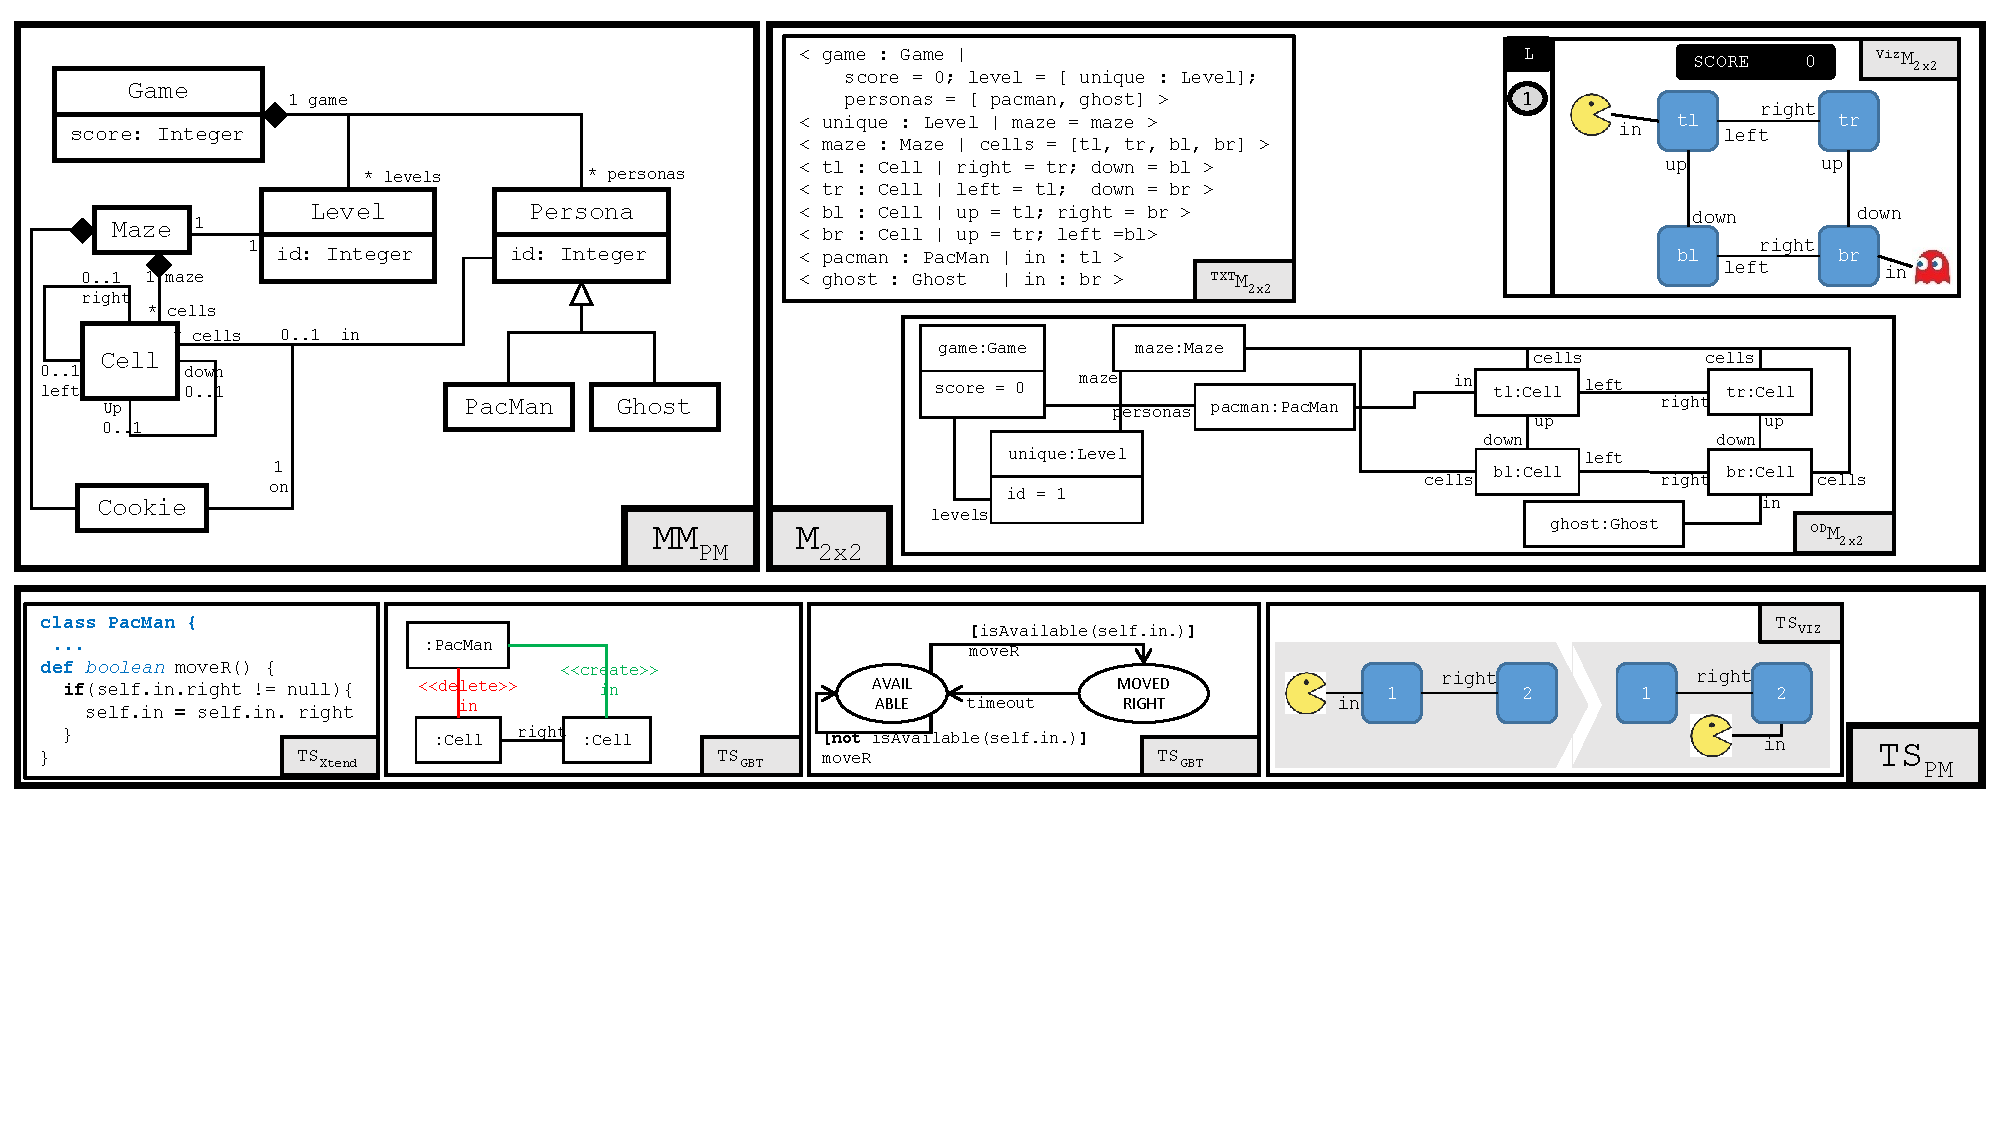
\includegraphics[width=\textwidth,clip, trim=0cm 5.5cm 0cm 0cm]{MM-M-T.pdf}
   \caption{Specifying a Pac-Man DSL: the DSL engineer create the metamodel 
   $\mathsf{MM}_{\mathsf{PM}}$; a modeller chooses a concrete syntax to create
   a simple model $\mathsf{M}_{\mathsf{2x2}}$; a MT designer specifies a transformation
   $\mathsf{TS}_{\mathsf{PM}}$ (only the \emph{\textsf{moveR}} MT unit is shown)}
   \label{fig:PacMan}
   \Description[<short description>]{<long description>}
\end{figure*}

\subsubsection{Execution}
\label{sec:Examples:PacMan:Execution}

The bottom compartment of \autoref{fig:PacMan} describes a simple rule 
\emph{\textsf{moveR}} (moving Pac-Man on a \textsf{Cell} at its right, if 
available) as part of the simulation MT specification $\mathsf{TS}_{\mathsf{PM}}$,
as part of $\mathsf{MM}_{\mathsf{PM}}$'s executable semantics. 
The first MT, $\mathsf{TS}_{\mathsf{Xtend}}$, uses metaprogramming 
(based on Xtend with GeMoC \cite{Leroy-Bousse-etAl:2017}). The next and last ones
are based on Graph Transformations: $\mathsf{TS}_{\mathsf{GBT}}$ relies on 
$^{\mathsf{OD}}\mathsf{M}_{\mathsf{2x2}}$ to express the rewriting (as would be 
expressed e.g. in Henshin \cite{Bill-Gabmeyer-Kaufmann-Seidl:2014}); 
while $\mathsf{TS}_{\mathsf{VIZ}}$ relies on $^{\mathsf{Viz}}\mathsf{M}_{\mathsf{2x2}}$
(as would be expressed e.g. in AtoMPM \cite{J:SyrianiVangheluwe:2013}). 
Finally, $\mathsf{TS}_{\mathsf{FSM}}$ presents an MT fragment expressed with 
a UML's Finite State Machine \cite{B:Rumbaugh-Jacobson-Booch:2004}. 
Note that all MT specifications (fragments) but $\mathsf{TS}_{\mathsf{Xtend}}$ 
present a graphical representation, showing that MT specifications may well be 
graphically visualised as well.

\subsubsection{Animations}
\label{sec:Examples:PacMan:Animations}

The PacMan game typically uses three kinds of animations for different situations:
\begin{description}
   \item[A \textsf{Persona} moves.] Typically, a specific animation could be attached
   to each movement, as they are traditionally encoded in different rules/operations
   (cf. e.g. \textsl{moveR} as specified in \autoref{fig:PacMan}, but also 
   \textsl{moveL}, \textsl{moveU} and \textsl{moveD} for moving left, up and down).
   Depending on whether the MTL allows using abstract classes (which would be 
   \textsf{Persona} here) for MT specification, these rules/operations may need 
   to be duplicated. 
   
   \item[\textsf{PacMan} eats a \textsf{Cookie}.] This occurs when \textsf{PacMan} is on a \textsf{Cell}
   that contains a \textsf{Cookie}, making it disappear and triggering a 
   \textsf{Score} update.
   
   \item[\textsf{PacMan} is eaten by a \textsf{Ghost}.] This occurs when 
   \textsf{PacMan} is on the same \textsf{Cell} as a \textsf{Ghost}, which may occur
   by either \textsf{Persona} making a move to an already occupied \textsf{Cell}.
\end{description}
To summarise, we would have to define four different animations to fully animate
the \textsf{PacMan} \DSL:
\begin{description}
   \item[PM.1] The \textsf{Persona} disappears from one \textsf{Cell} and reappears
   on another (adjacent) \textsf{Cell}.
   
   \item[PM.2] Assuming \textsf{PacMan} is on a \textsf{Cell} containing a \textsf{Cookie},
   the \textsf{Cookie} disappears.
   
   \item[PM.3] The \textsf{Score} is updated by a given increment. 

   \item[PM.4] Assuming \textsf{PacMan} and a \textsf{Ghost} are on the same
   \textsf{Cell}, \textsf{PacMan} disappears.
\end{description}
Note that those animations are not completely unrelated. First, \textbf{PM.2} and
\textbf{PM.3} need to be conducted sequentially quickly enough to not notice a
time gap. Second, \textbf{PM.2} and \textbf{PM.4} appear to be very similar in
nature: they both assume that two objects are located on the same \textsf{Cell} 
before making one of them disappear.

\subsection{\textsf{FSM}: A \DSL for Finite-State Machines}
\label{sec:Examples:FSM}

Finite State Machines (FSM) represent a common \DSL for capturing state-based 
behaviour of various biological, but also computational domains (e.g. Turing 
Machines, but also Chomsky's Regular Grammars, among others). This Section considers
FSMs that are simplified in various ways: in particular, we only consider a
word acceptance semantics where transitions do not contain guards and triggers are
reduced to their simplest expression, namely simple strings.

\subsubsection{Specification}
\label{sec:Examples:FSM:Specification}

\begin{figure}%
   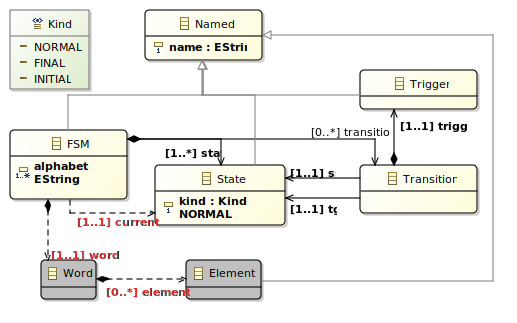
\includegraphics[width=\columnwidth]{FSM}%
   \caption{A metamodel for Finite State Machines.}%
   \label{fig:FSM_MM}%
\end{figure}


\autoref{fig:FSM_MM} (top) specifies the metamodel of the Finite State Machine \DSL. 
An \textsf{FSM} is composed of \textsf{State}s identified by a \textsf{name}, and
\textsf{Transition}s that contain a simple \textsf{Trigger}, specified as 
\textsf{name}d event. \autoref{fig:FSM_M} depicts a simple model consisting of 
three \textsf{State}s and three \textsf{Transition}s, to recognise the regular 
expression $\mathtt{(a\cdot b)^\star\ b}$. 

We assume the classical visual representation for \textsf{FSM}: a \textsf{State}
is represented by a circle labelled with its \textsf{name}; and a 
\textsf{Transition} is represented by an arrow pointing to its \textsf{tgt} and 
carrying the \textsf{Trigger}'s name as a label. We represent the \textsf{current}
\textsf{State} by surimposing a red rounded form (that we call \emph{token}) over
the corresponding \textsf{State} (cf. \autoref{fig:FSM_M}).


\subsubsection{Execution}
\label{sec:Examples:FSM:Execution}

We adopt a \emph{word-recognising} semantics encoded in a transformation called
\textsf{accept} that reads a \textsf{Word} and traverses the \textsf{FSM}. A 
\textsf{Word} is accepted iff the \textsf{current} \textsf{State} of the \textsf{FSM}
is \textsf{FINAL} when the \textsf{Word} becomes empty.

\subsubsection{Animations}
\label{sec:Examples:FSM:Animations}

Typically, \textsf{accept} is implemented using a sub-transformation 
\textsf{fire(e : Element) : State [0..1]} that determines which \textsf{State} 
to update to when consuming an \textsf{Element} \textsf{e}, making it a good 
candidate for four different animations, when \textsf{fire} returns an actual 
\textsf{State}:
\begin{description}
   \item[FSM.1] The token disappears from the \textsf{current} \textsf{State} and
   reappears inside the updated \textsf{current};
   \item[FSM.2] The token disappears from the \textsf{current} \textsf{State}, and
   slides along the entire arrow of the fired \textsf{Transition}, then appears in
   the updated \textsf{current};
   \item[FSM.3] The token disappears from the \textsf{current} \textsf{State}, the
   arrow of the fired \textsf{Transition} blinks in red for 2 seconds, then the 
   token reappears in the updated \textsf{current}.
\end{description}


\begin{figure}[t]%
   \centering
   \begin{subfigure}[b]{0.45\columnwidth}
      \centering
      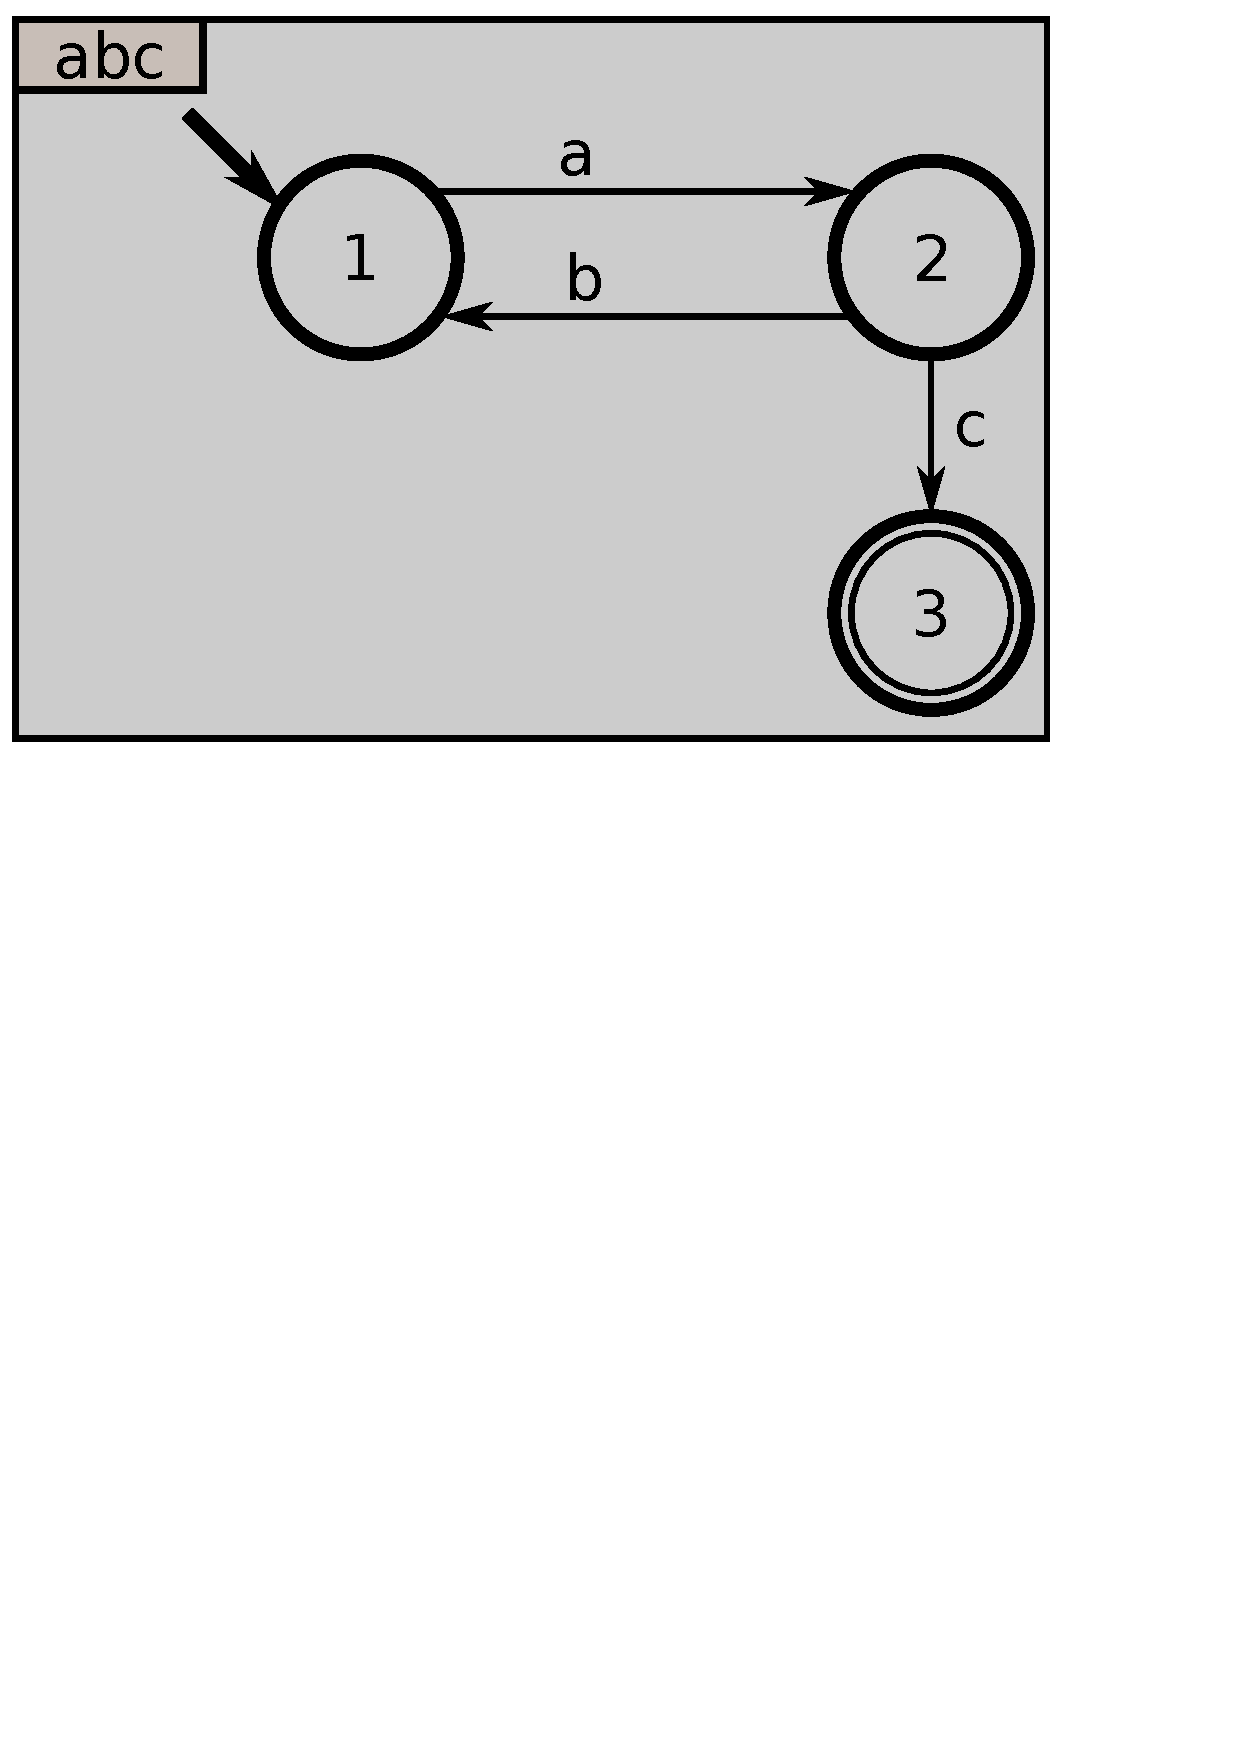
\includegraphics[width=\columnwidth, clip, trim=0cm 17cm 3cm 0cm]{FSM_M.pdf}%
      \caption{Editing \textsf{abc} to obtain a 3-state/3-transition FSM model: 
      states \textsf{1} and \textsf{3} are respectively \textsf{INITIAL} and 
      \textsf{FINAL}.}
      \label{fig:FSM:Model:Edition}
   \end{subfigure}
   \hfill
   \begin{subfigure}[b]{0.45\columnwidth}
      \centering
      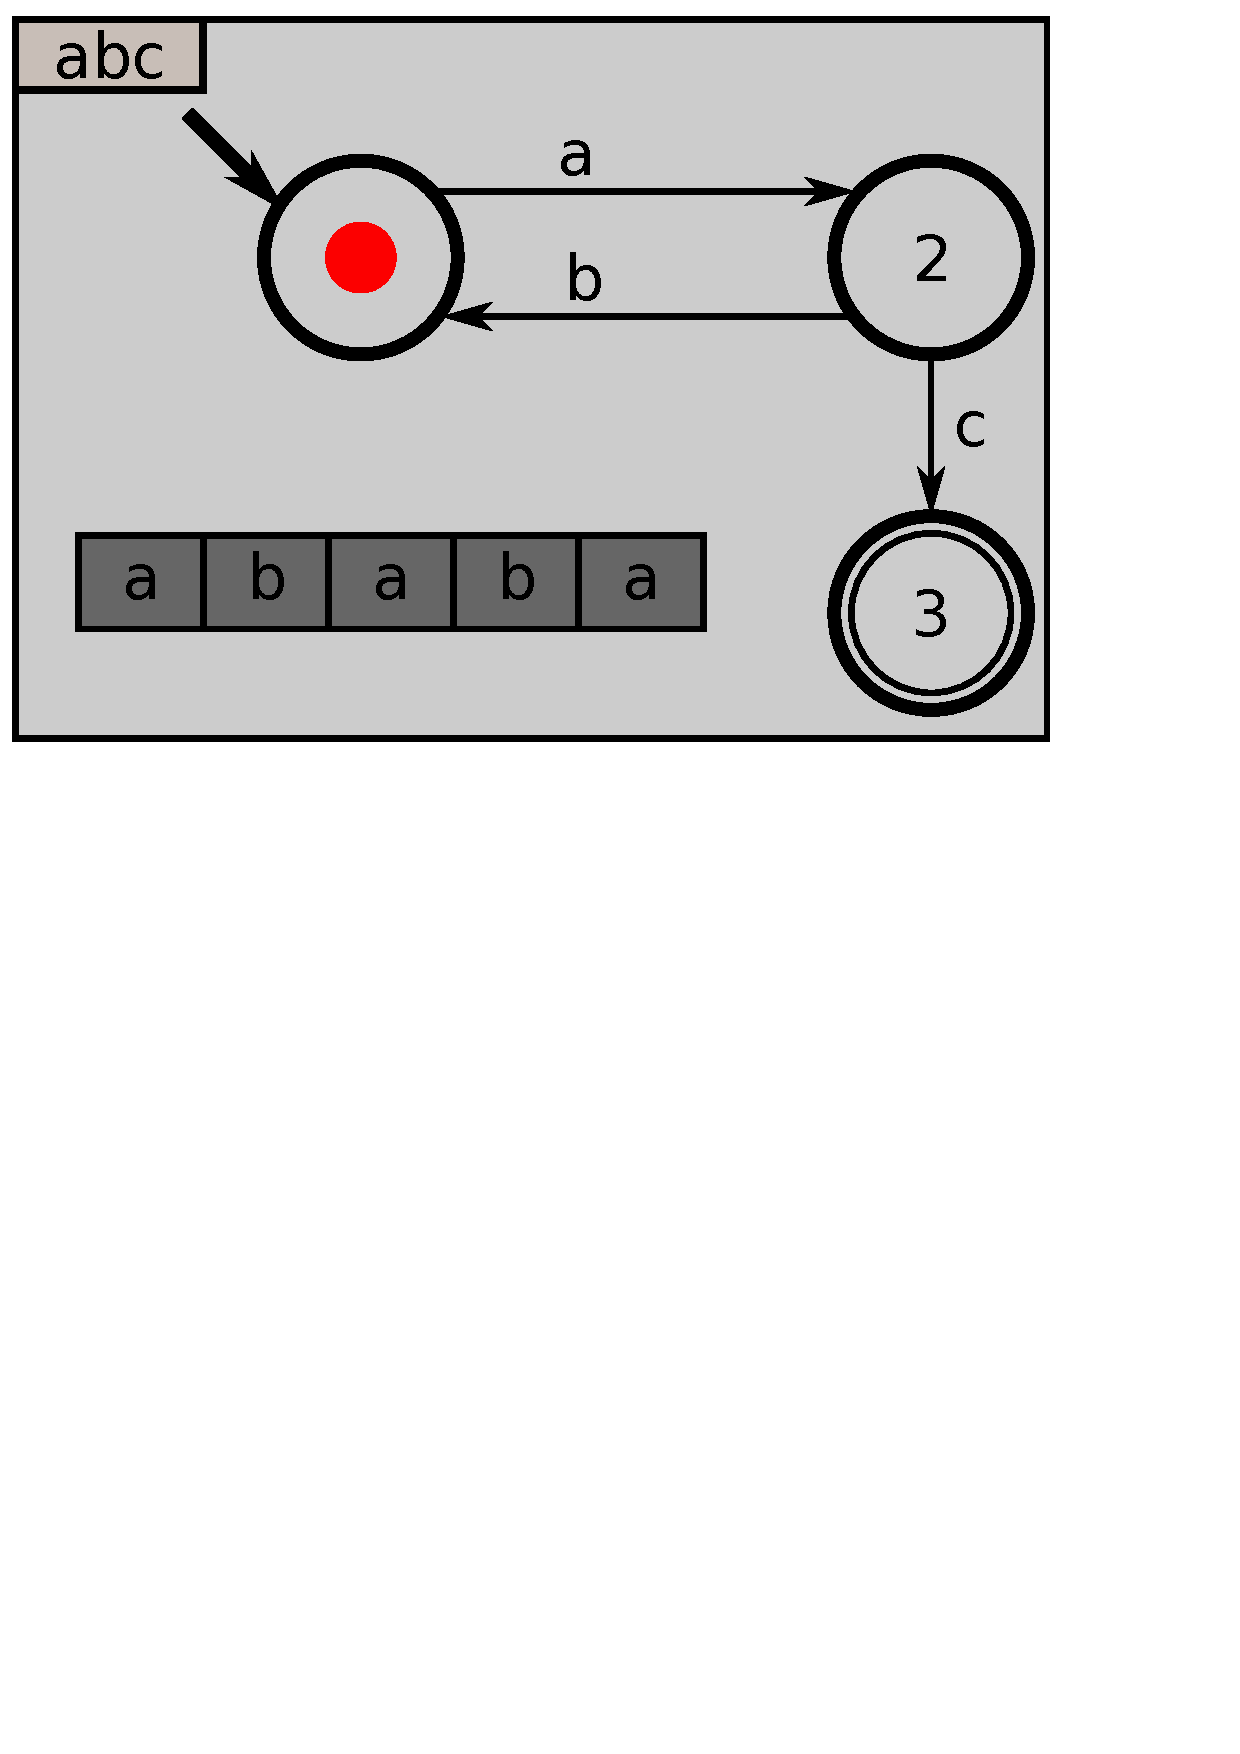
\includegraphics[width=\columnwidth, clip, trim=0cm 17cm 3cm 0cm]{FSM_MX.pdf}%
      \caption{Starting executing \textsf{abc}: the \textsf{current} 
      \textsf{State} is overlayed with a red token, and attempting to accept the
      word \textsf{ababa}.}
      \label{fig:FSM:Model:Execution}
   \end{subfigure}
  
   \vskip\baselineskip
   \begin{subfigure}[b]{0.45\columnwidth}
      \centering
      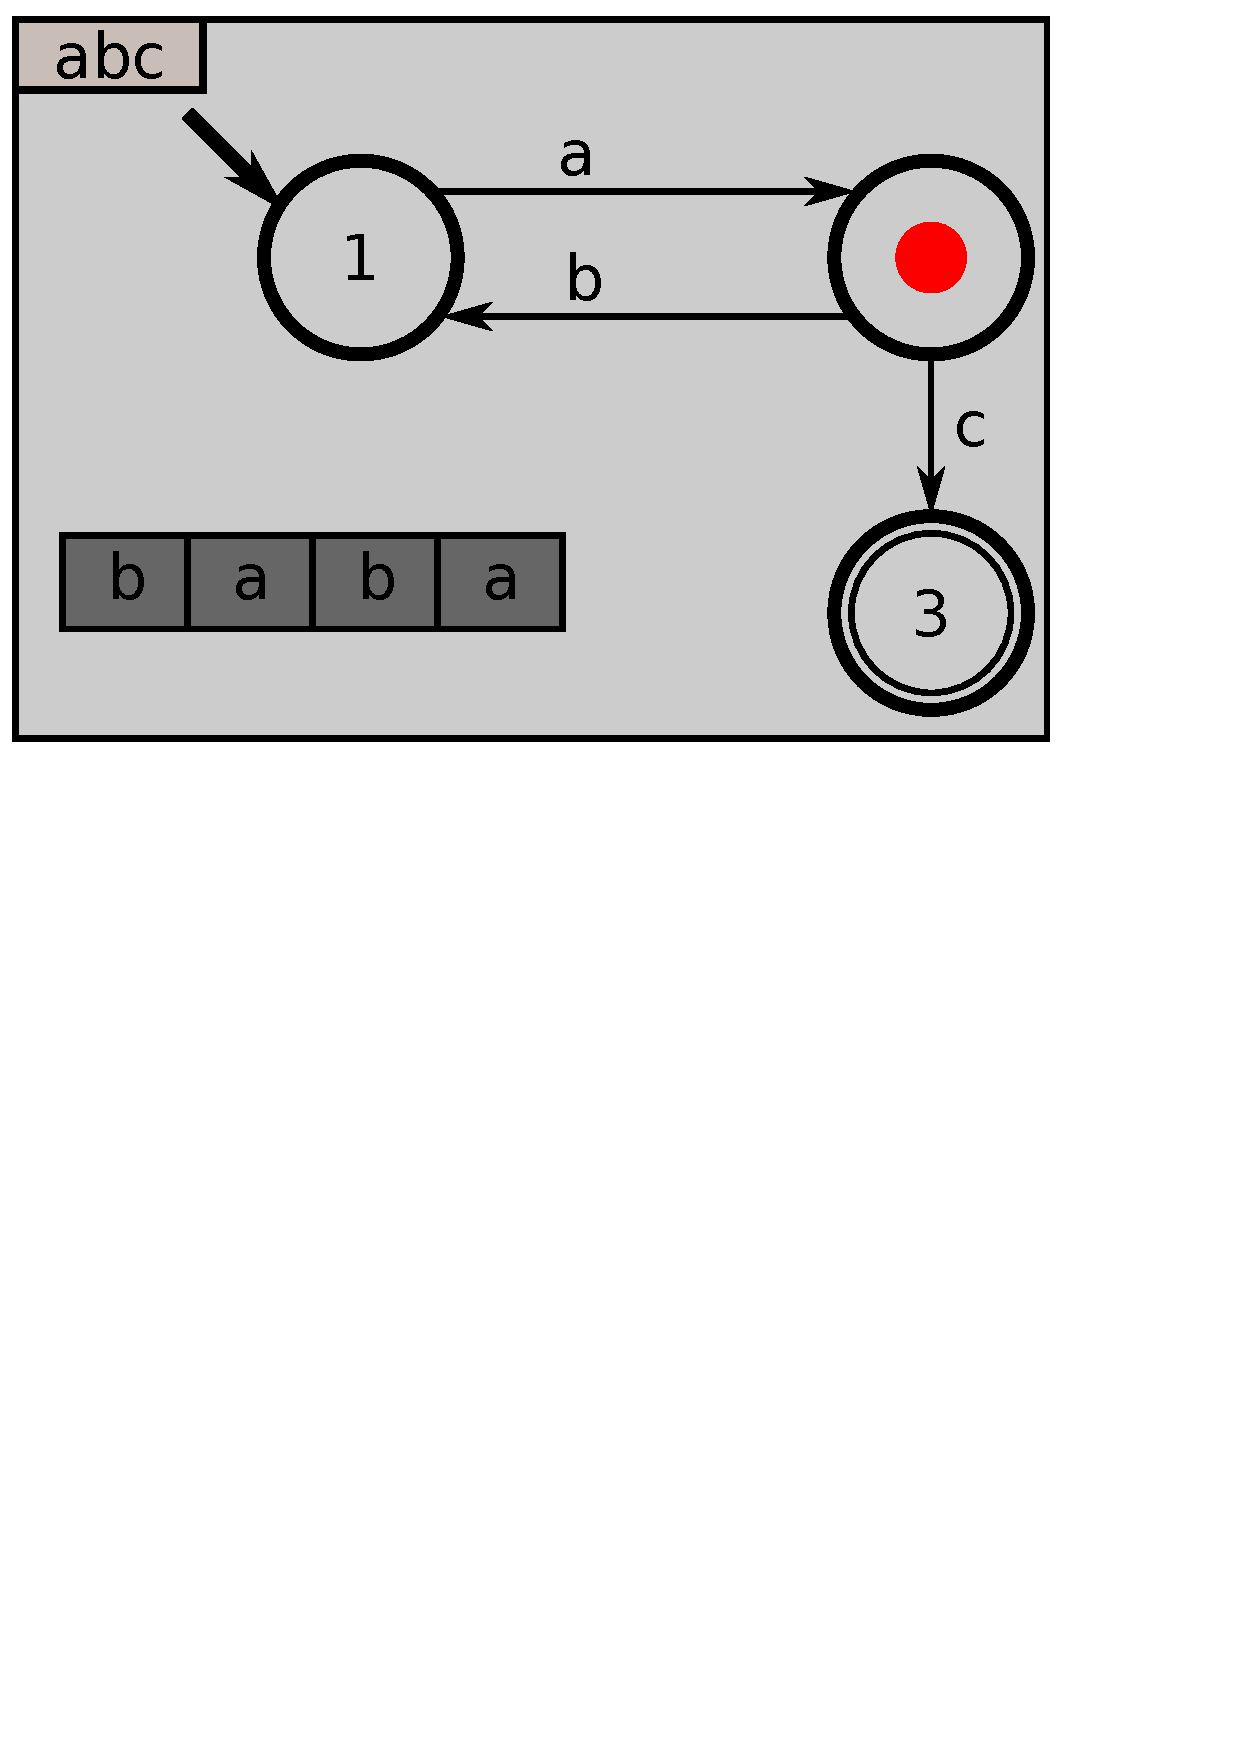
\includegraphics[width=\columnwidth, clip, trim=0cm 17cm 3cm 0cm]{FSM_MA11.pdf}%
      \caption{\textbf{Animation FSM.1:} The first execution step moves the token in
      \textsf{State} 2 (while consuming the first \textsf{Element} \textsf{a}).}
      \label{fig:FSM:Model:Animation:FSA1.1}
   \end{subfigure}
   \hfill
   \begin{subfigure}[b]{0.45\columnwidth}
      \centering
      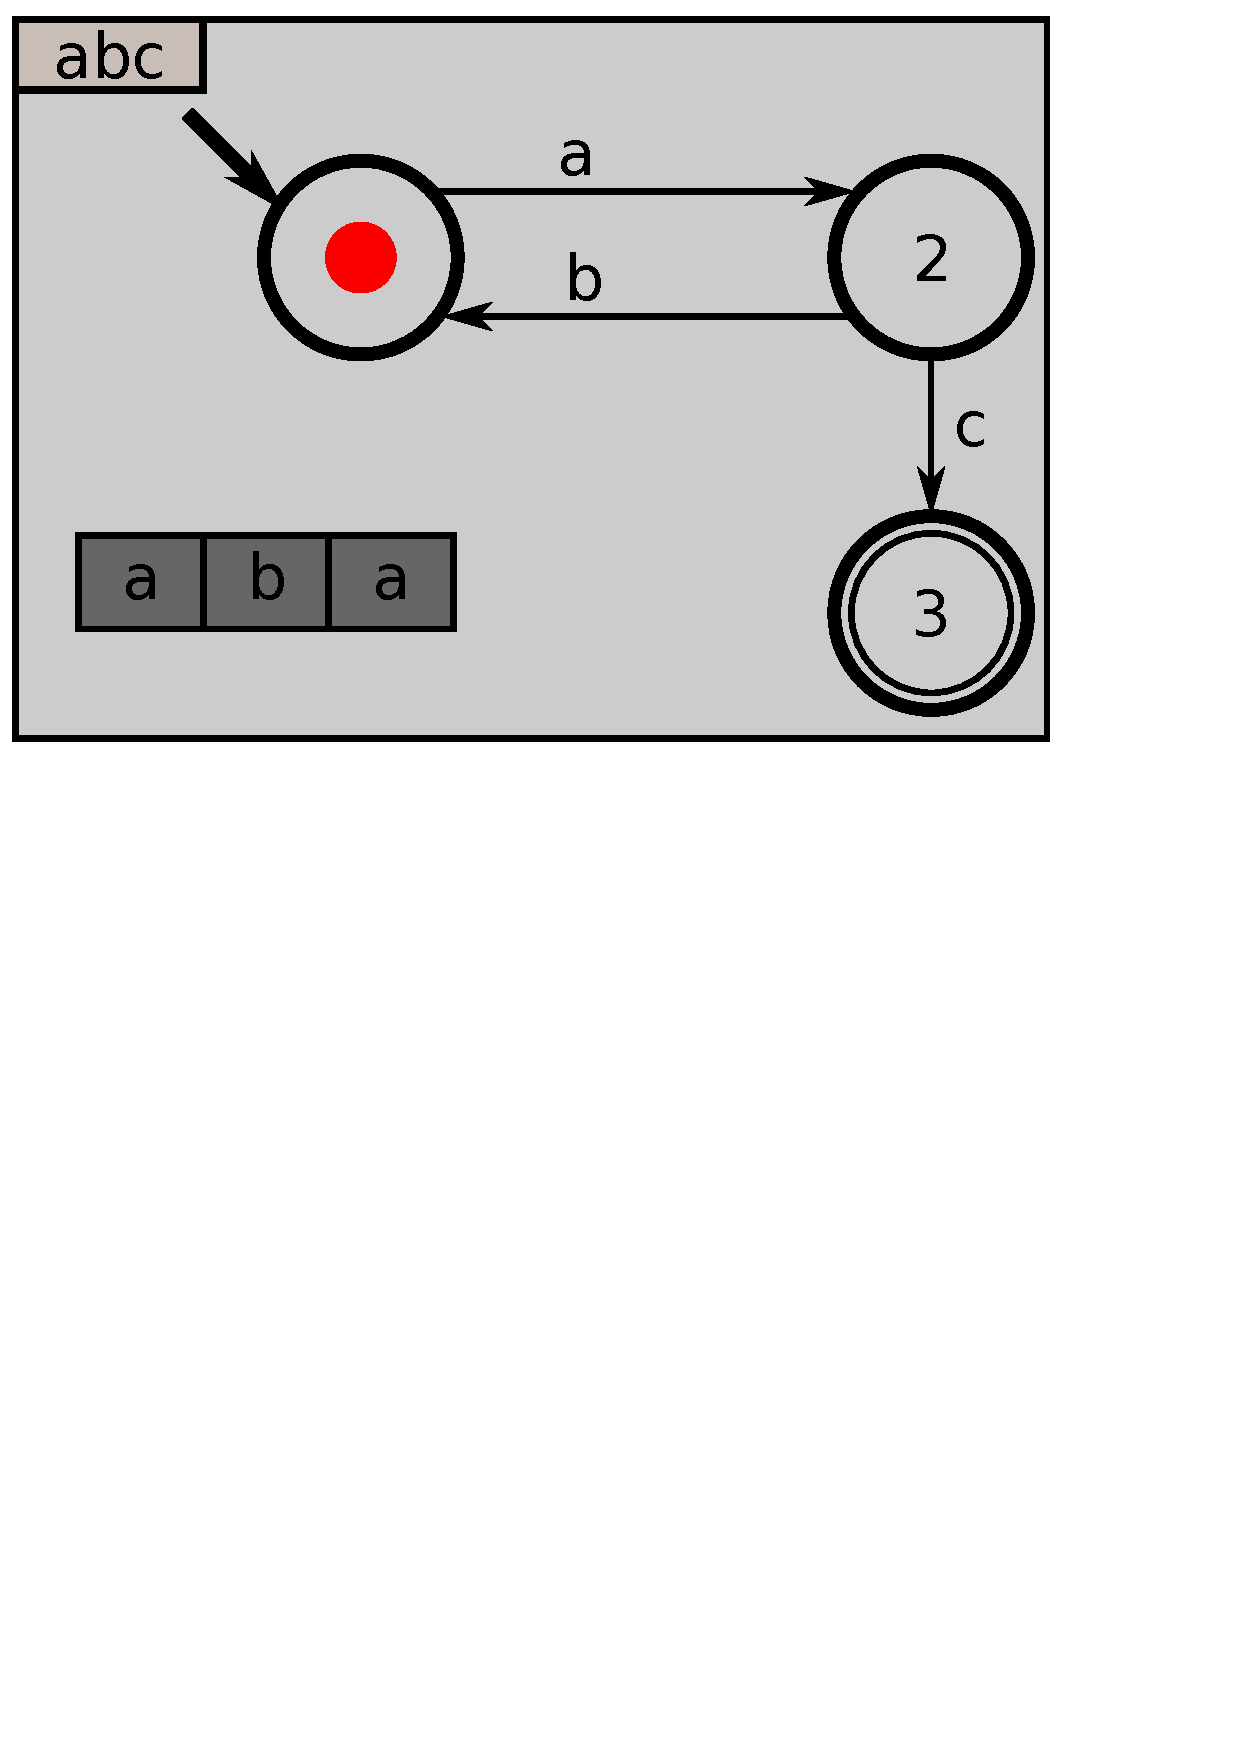
\includegraphics[width=\columnwidth, clip, trim=0cm 17cm 3cm 0cm]{FSM_MA12.pdf}%
      \caption{\textbf{Animation FSM.1:} The second execution step moves the token 
      back in \textsf{State} 1 (while consuming \textsf{b}).}
      \label{fig:FSM:Model:Animation:FSA1.2}
    \end{subfigure}
 
    \vskip\baselineskip
    \begin{subfigure}[t]{0.45\columnwidth}
      \centering
      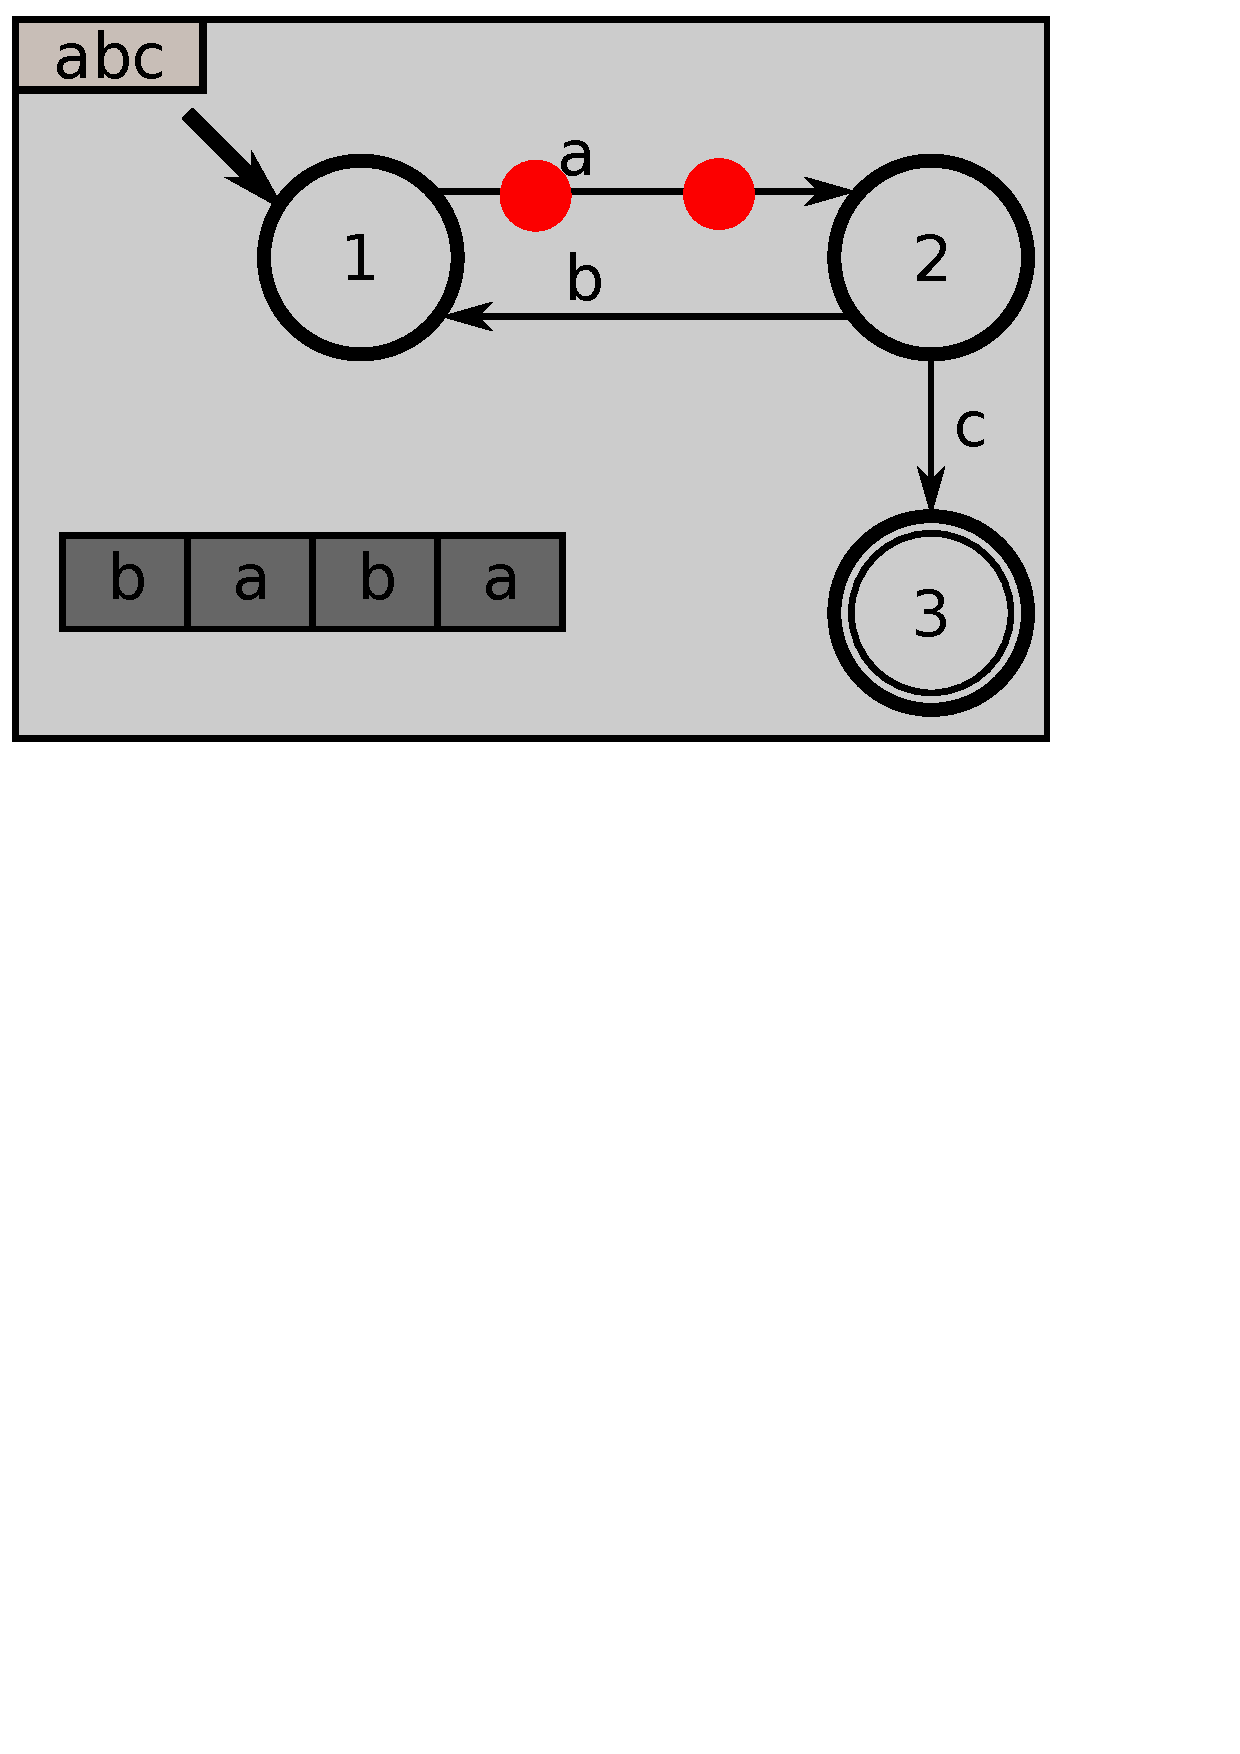
\includegraphics[width=\columnwidth, clip, trim=0cm 17cm 3cm 0cm]{FSM_MA21.pdf}%
      \caption{\textbf{Animation FSM.2:} The first phase of the animation slides
      token along the \textsf{Transition} \textsf{a} (represented here in two 
      different positions to reproduce the animation's visual effect).}
      \label{fig:FSM:Model:Animation:FSA2.1}
    \end{subfigure}
    \hfill
    \begin{subfigure}[t]{0.45\columnwidth}
      \centering
      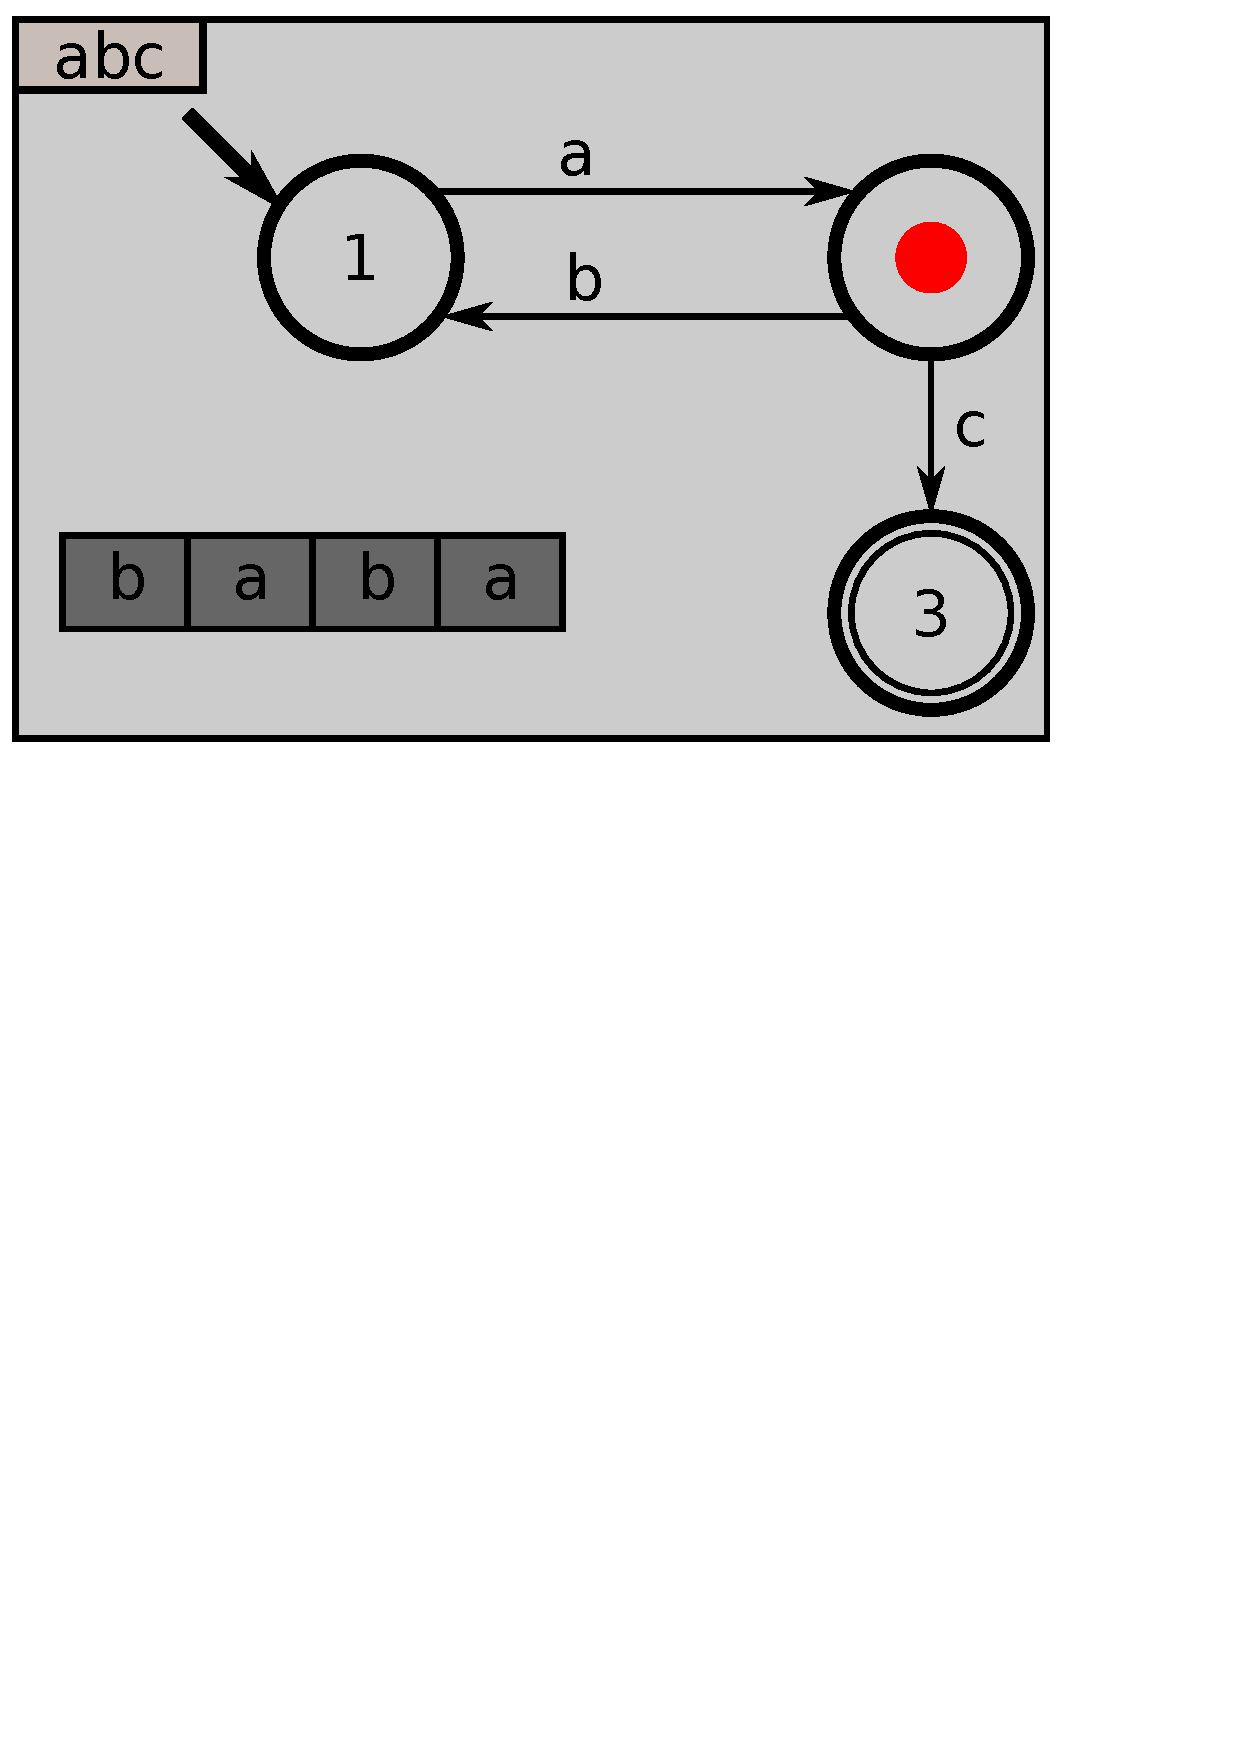
\includegraphics[width=\columnwidth, clip, trim=0cm 17cm 3cm 0cm]{FSM_MA22.pdf}%
      \caption{\textbf{Animation FSM.2:} The second phase of the animation makes
      the token appears in \textsf{State} 2, after consuming \textsf{b}.}
      \label{fig:FSM:Model:Animation:FSA2.2}
    \end{subfigure}

    \vskip\baselineskip
    \begin{subfigure}[t]{0.45\columnwidth}
      \centering
      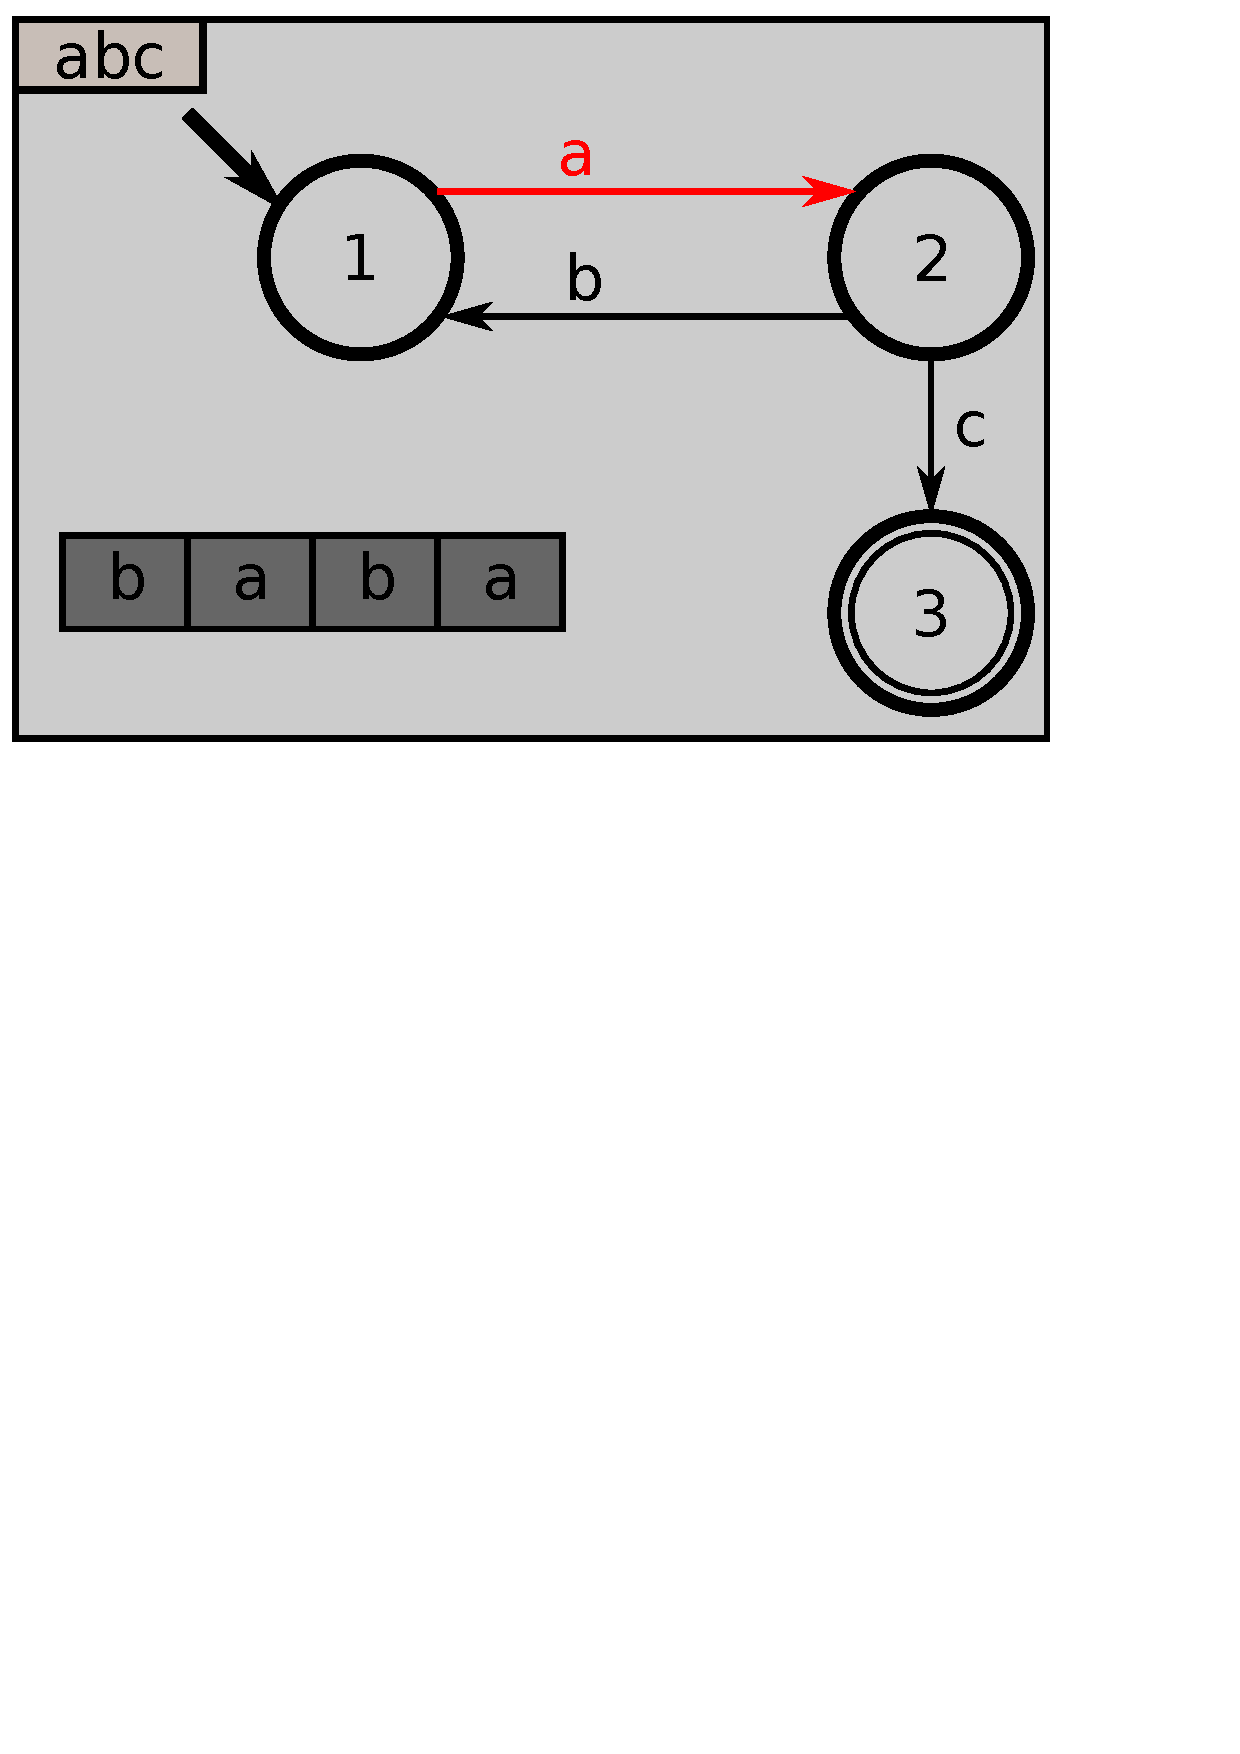
\includegraphics[width=\columnwidth, clip, trim=0cm 17cm 3cm 0cm]{FSM_MA31.pdf}%
      \caption{\textbf{Animation FSM.3:} The first phase of the animation highlights
      \textsf{Transition} \textsf{a} in red (as well as its \textsf{Trigger}).}
      \label{fig:FSM:Model:Animation:FSA2.3}
    \end{subfigure}
    \hfill
    \begin{subfigure}[t]{0.45\columnwidth}
      \centering
      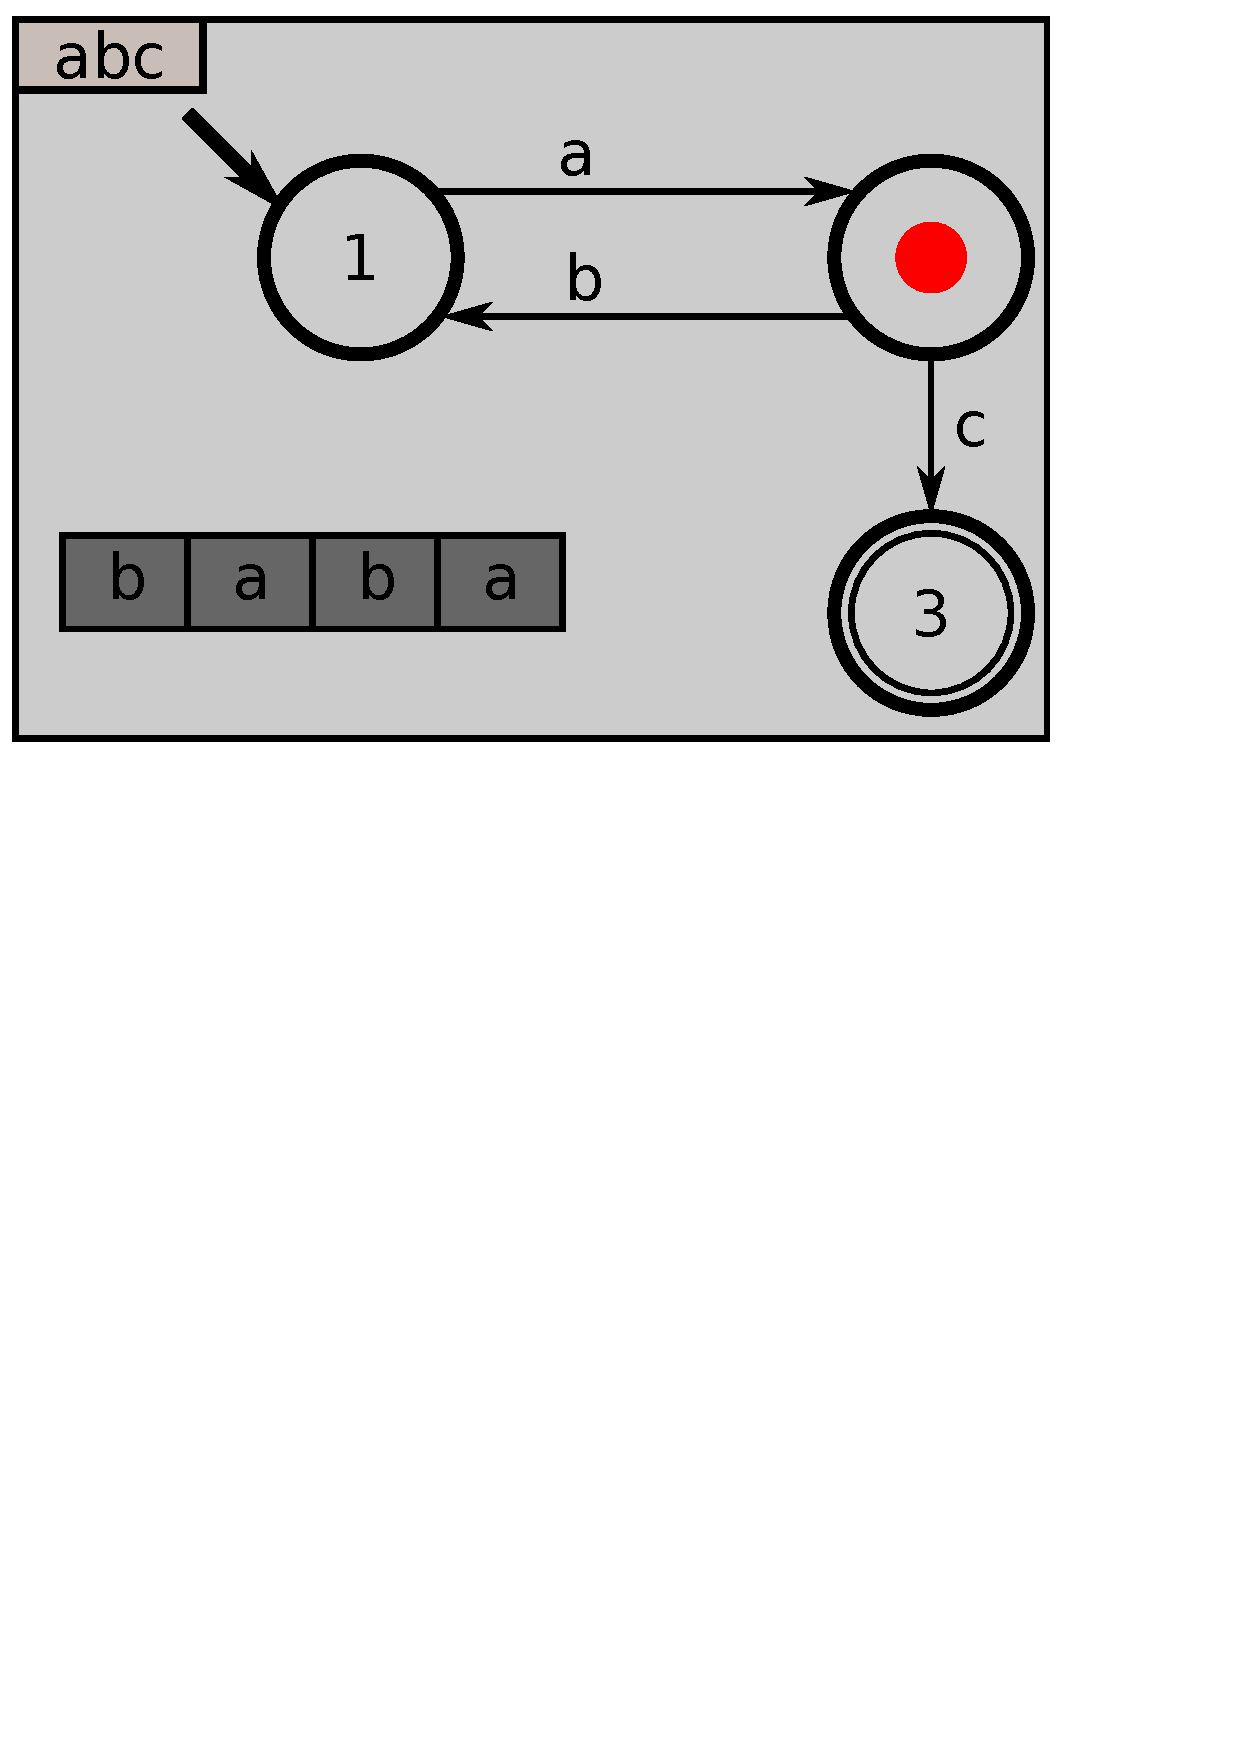
\includegraphics[width=\columnwidth, clip, trim=0cm 17cm 3cm 0cm]{FSM_MA22.pdf}%
      \caption{\textbf{Animation FSM.3:} The second phase of the animation makes
      the token appears in \textsf{State} 2, after consuming \textsf{b}.}
      \label{fig:FSM:Model:Animation:FSA2.4}
    \end{subfigure}

  \caption{\textsf{abc}: a simple model of an FSM conforming to the specification
   in \autoref{fig:FSM_MM}, and some associated animations for its execution 
   (cf. \S \ref{sec:Examples:FSM:Animations} for their specification.)}%
   \label{fig:FSM_M}%
\end{figure}


\subsection{\textsf{PN}: A \DSL for (Simple) Petri Nets}
\label{sec:Examples:PN}

\subsubsection{Specification}
\label{sec:Examples:PN:Specification}

\subsubsection{Execution}
\label{sec:Examples:PN:Execution}

\subsubsection{Animations}
\label{sec:Examples:PN:Animations}






\subsection{Concrete Syntax (CS)}
\label{sec:CS}

The first challenge, Concrete Syntax (CS), is related to a \DSML's metamodel 
\textsf{MM} through two transformations:

$$ \mathsf{MM} \xrightleftharpoons[\mathrm{parsing}\phantom{MM}]{\phantom{MM}\mathrm{rendering}} \mathsf{CS}$$

In syntax-directed editing, \emph{parsing} is not necessary because models
are created by relying on the syntax, thus preventing ill-models. On the other hand,
\emph{rendering} is crucial for representing a model when appropriate, but
it also represents the anchor for animation. 


Having explicit MTs between \textsf{MM} and \textsf{CS} assumes indeed that 
\textsf{CS} is explicitly metamodelled: following the \MDE methodology, such
a \DSL should cover the definition of visual representations (geometric shapes as
well as various data structure representations such as tables, graphs, etc.),
but also the ability to define the rendering relationship, i.e. patterns associating
\textsf{MM}'s metamodel elements with \textsf{CS}'s elements.
We identified at least four challenges:

\begin{figure}[t]%
   \centering
   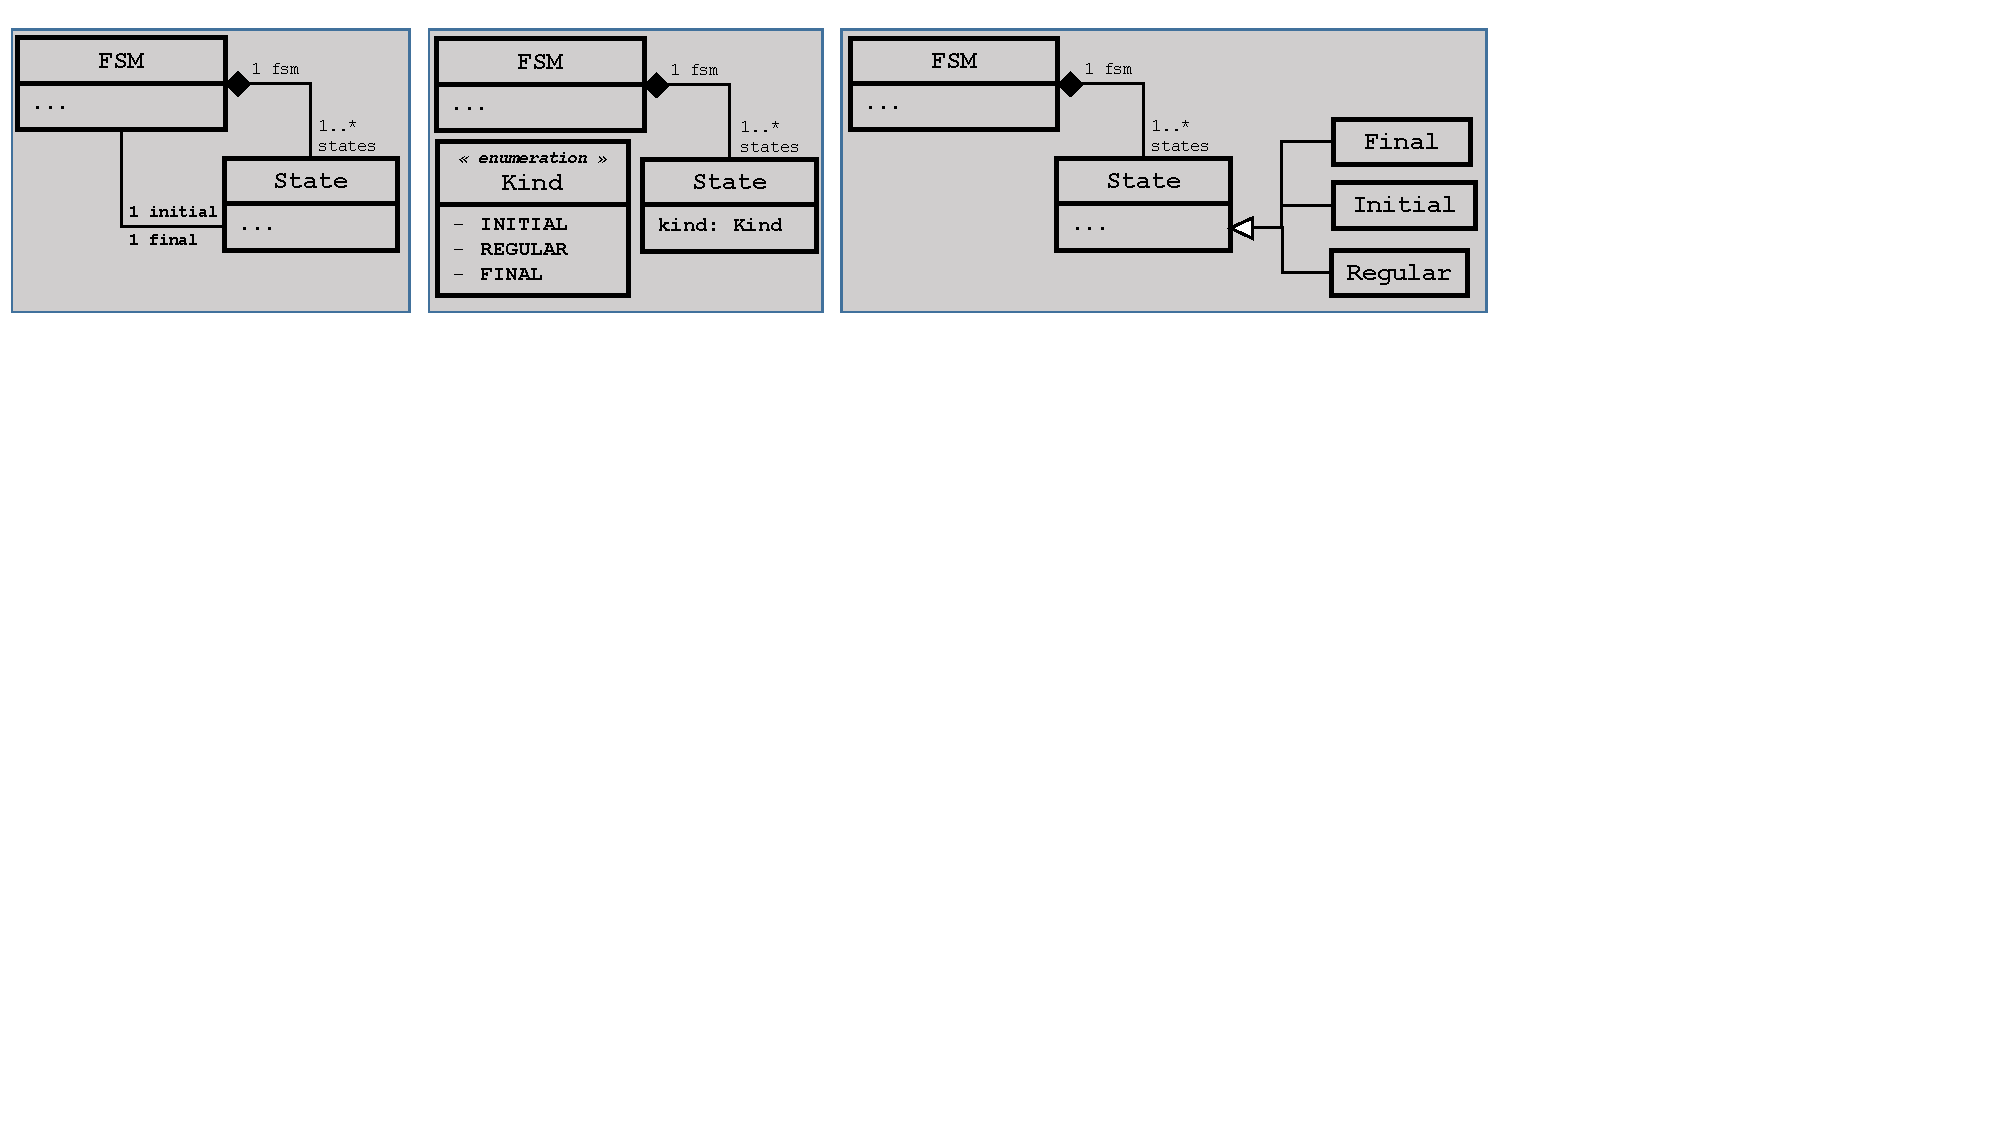
\includegraphics[width=\columnwidth,clip, trim=0cm 13.8cm 8.3cm 0.2cm]{FSM-Initial}%
   \caption{Modelling a \textsf{State} in \textsf{FSM}: with explicit references
   \texttt{initial} and \texttt{final} (left); with a distinguishing property 
   \texttt{kind} (middle); and with inheritance (right).}%
   \label{fig:FSM-Initial}%
   \Description[Different ways of modelling \textsf{FSM}'s \textsf{State}s.]{%
   A \textsf{State} is modelled with explicit references, with a distinguishing 
   property in \textsf{State} specifying, with an enumeration, the different 
   \textsf{kind}s, and with inheritance.}
\end{figure}

\begin{description}
   \item[CS.1. Providing \emph{simple} visualisation of data struc\-tures.]
   Pro\-vi\-ding configurable representations for common data structures such as
   (multi-column) tables, graphs, sets and lists present the benefit of rapidly
   presenting information from a model. This ability should rely on queries to
   identify, and eventually modify, the elements of the model used for ``populating''
   such structures. 

	\item[CS.2. Providing \emph{complex} rendering patterns.]
   Consider the (partial) meta\-models in \autoref{fig:FSM-Initial} that
   specify the \emph{initial} \textsf{State} in four different ways: by referencing
   to the appropriate \textsf{State} among those available, by characterising each \textsf{State} with
   a property \textsf{kind}, or by using type inheritance. Many tools would only
   support the latter, because they essentially only allow to 
   associate various icons to classes. This approach is too simplistic and forces
   metamodel designers to tweak their metamodels towards MA, introducing yet another
   metamodel specialisation (as it is already the case for model editing and
   model analysis, among others). Complex rendering patterns should allow to freely
   associate visual counterparts to various combinations and values of metamodel
   elements.
   
   \item[CS.3. Integrating ``insideness'' \emph{natively}] We call \emph{insideness}
   the visual equivalent of \emph{containment} in metamodelling, i.e. the ability
   to uniquely put elements \emph{inside} inside a container so that elements 
   inside disappear along with the container's removal. This feature presents two
   advantages. First, it would allow to natively handle common situations like 
   including text inside a shape (e.g. displaying a \textsf{State}'s name within
   the circle for an \textsf{FSM}) and then treat them in an universal manner. 
   Second, if the feature is customisable, it would enforce a natural semantics
   graphically with an expected behaviour. 
   
   \item[CS.4. Providing ``snapping'' capabilities] Snapping helps precise\-ly arrange
   graphical elements by ``gluing'' them to a specific target, e.g. a canva's
   boundary, a grid, or points on objects. 
      
   \item[CS.6. Supporting animations natively.] Having at disposal a \DSL
   for defining CSs brings the ability to \emph{visually} render metamodels, but
   does not guarantee the ability to perform animation. For that, the \DSL should
   natively support the fast update of visual features that compose the CS (e.g.,
   the position, size, color, type of line for an \textsf{FSM}'s 
   \textsf{Transition}).      
\end{description}




\balance
\bibliographystyle{plainnat}
\bibliography{./MLE}
\end{document}
